\documentclass[conference]{IEEEtran}
\IEEEoverridecommandlockouts
% The preceding line is only needed to identify funding in the first footnote. If that is unneeded, please comment it out.
\usepackage{cite}
\usepackage{amsmath,amssymb,amsfonts}
\usepackage{algorithmic}
\usepackage{graphicx}
\usepackage{textcomp}
\usepackage{xcolor}
%\usepackage{booktabs}
\usepackage{tabularray}
\usepackage{flushend}
\UseTblrLibrary{booktabs}
\def\BibTeX{{\rm B\kern-.05em{\sc i\kern-.025em b}\kern-.08em
    T\kern-.1667em\lower.7ex\hbox{E}\kern-.125emX}}
\begin{document}

\title{Gamifying Cybersecurity:\\The CTF Challenges}

\author{\IEEEauthorblockN{Gergely Vakulya}
\IEEEauthorblockA{\small \textit{Alba Regia Technical Faculty} \\
\textit{Óbuda University}\\
\textit{Székesfehérvár, Hungary}\\
\textit{vakulya.gergely@amk.uni-obuda.hu}
}
\and
\IEEEauthorblockN{Helga Anna Albert-Huszár}
\IEEEauthorblockA{\small \textit{Alba Regia Technical Faculty} \\
\textit{Óbuda University}\\
\textit{Székesfehérvár, Hungary}\\
\textit{albert.huszar.helga@amk.uni-obuda.hu}
}
}

\maketitle

\begin{abstract}
Cybersecurity is becoming increasingly critical in today's digital landscape,
  yet it remains challenging to enter the field due to its inherently complex
  nature, requiring expertise across a wide range of specialized areas. This
  paper explores the use of Capture the Flag (CTF) challenges as a gamified
  method for enhancing cybersecurity education and skill development. By
  integrating real-world scenarios into a competitive format, CTF challenges
  encourage participants to apply their knowledge in dynamic, problem-solving
  environments. We analyze various CTF challenge categories, and discuss their
  effectiveness in fostering critical cybersecurity skills.
\end{abstract}

\begin{IEEEkeywords}
cybersecurity, linux, forensics, cryptography
\end{IEEEkeywords}

\section{Introduction}

Education is increasingly shifting from traditional classroom settings to
virtual environments, necessitating the development of new, interactive
modalities to capture learners' attention effectively. As technology advances,
educational approaches must evolve to engage students more dynamically,
leveraging tools like gamification, multimedia content, and collaborative
platforms.
These methods not only enhance learning experiences but also
accommodate diverse learning styles, making education more accessible and
effective for a wider audience.

Virtual education environments
% Berti cikkei, virtualis oktatas
\cite{gyorok2014}
\cite{safar2019}
\cite{beszedes2023}
facilitate real-time interaction between
students and educators, promoting active participation and critical thinking.
By integrating elements such as simulations, online discussions, and hands-on
projects, educators can create immersive learning experiences that foster
deeper understanding and retention of material.

One crucial field that warrants focused educational efforts is cybersecurity.
As cyber threats become more sophisticated and pervasive, it’s essential to
equip learners with the skills and knowledge to defend against them. One
effective and engaging approach to teaching cybersecurity is through Capture
the Flag (CTF) challenges. These competitions provide a hands-on learning
experience where participants solve real-world problems and exploit
vulnerabilities in controlled environments.
%Cybersecurity oktatas
\cite{rahman2020}
%Cybersecurity az egyetemen
\cite{schneider2013}

The name of CTF comes fom the traditional game of capture the flag. It
involves two teams, each tasked with
defending their own flag while attempting to capture the opposing team’s flag.
In CTF challenges, however, the 'flag' typically takes the form of a hidden or
encrypted string (such as a password), which is securely protected.
Successfully capturing the flag serves as proof that the player has overcome
the challenge by breaching the system's defenses or solving the puzzle.

CTF challenges are based in information technology, often demanding a deep
understanding of various technologies that extend well beyond traditional
software development. They are designed to simulate real-world security
challenges, helping participants understand the tactics used by both attackers
and defenders. This practical insight is invaluable in understanding modern
security threats.

CTF challenges are typically organized into distinct categories, with the most
common being binary exploitation, reverse engineering, cryptography, web
technologies, and digital forensics. Each category focuses on a specialized
area, requiring participants to apply specific skills and knowledge to solve
the associated problems. There are challenges that demand expertise across multiple
fields, while others don't fit into any of the afore mentioned categories.

These challenges are part of a CTF event or competition, usually held yearly.
While some of them are in-pearson events, the popular ones are online competitions.
A CTF competition consist of multiple challenges from varying categories. They
are usually team-based, encouraging participants to work together to solve
complex problems. Solving challenges can build teamwork and it can be to a
team's advantage that each member approaches the same problem differently, not
to mention that a team typically consists of members who are good at different
challenge categories.

The competitive nature of events keeps participants motivated to
improve and learn more as they strive to outperform other teams. Solving
complex problems can bring satisfaction, boost confidence and inspire further
learning and participation in cybersecurity.

The challenges from past years are available to solve online to develop the
skills necessary to participate or to practice for the next competition. There are
leaderboards to track the progress as well. As a result it becomes easy to
enter the field of cybersecurity.

Unlike traditional classroom learning,
CTF challenges provide hands-on
experience, making learning more engaging and effective. Some challenges
require writing a writeup, which is a document describing in detail the process
of solving the problem. Writeups are important learning resources for people
who could not solve that particular challenge or new to cybersecurity. It also
broadens one's mind to see how others solved the same challenge.

%CTF problems are not only good for practicing, but they are competitive

%time, leaderboard, utólag elérhető.

%Vannak online es jelenleti esemenyek
%is, illetve elerhetoek az elozo feladatok. Lehet csapatos, vagy egyeni.
%A csapat osszetartozasat is jol erositi. Tobb ember tobb nezopontbol maskepp lathatja.
%Writeup: Ebben egy csapat, vagy szemely megoldasa van reszletesen leirva.

\section{CTF events}
\label{sec-ctf-events}

\subsection{Google CTF}

Google CTF is an annual, entirely online Capture the Flag (CTF) competition hosted by Google,
aimed at both beginner and advanced participants. The event is designed to
foster interest in cybersecurity and challenge individuals to solve a variety
of technical problems related to hacking, cryptography, and exploitation. It
has become one of the most recognized CTF events in the cybersecurity
community.

Google CTF features both a beginner-friendly and advanced division, catering to
participants with varying levels of expertise. The beginner track, sometimes
called "Beginner's Quest," allows newcomers to ease into cybersecurity by
solving easier problems. Meanwhile, the advanced track pushes experienced
hackers to their limits, tackling complex challenges across multiple
disciplines.

\subsection{PicoCTF}

picoCTF is one of the largest CTF competitions designed
primarily for middle and high school students, but it’s open to anyone
interested in learning cybersecurity. It was launched in 2013 \cite{zhang2013}
by Carnegie Mellon
University’s CyLab Security and Privacy Institute, and continues to be organized annually.

What sets picoCTF apart from other CTF competitions is its educational focus.
Unlike many CTFs, which are primarily competitive, picoCTF is designed to teach
participants fundamental security concepts while they compete. It features a
learning environment called picoGym, where users can practice their skills on
challenges from previous years at their own pace. This flexible,
learn-as-you-go format is especially useful for beginners and educators looking
to integrate cybersecurity into their curricula.

\subsection{Hungarian Cyber Security Challenge}

The Hungarian Cyber Security Challenge (HCSC) is Hungary’s premier
cybersecurity competition, organized annually by the National Cyber Security
Center. Being Open to Hungarian citizens aged 16 and above, the event is
aimed to identify and promote the next generation of
cybersecurity talent. 

Unlike most traditional CTF competitions, there are some specific challenges
where participants are required to provide detailed documentation, known as
''writeups'', explaining how they solved the problem and captured the flag. These
writeups serve as comprehensive reports that outline the methods and tools used
to exploit vulnerabilities and provide step-by-step explanations of the
problem-solving process.

Another unique aspect of this event is that the final rankings are not solely
determined by the points participants accumulate during the competition. In
addition to the scores, the organizers place significant weight on the quality
of the participants' writeups and the methods they used to solve the
challenges. This approach ensures that creativity, technical depth, and
problem-solving strategies are recognized alongside mere point accumulation.
By evaluating the techniques and documentation provided in the writeups, the
organizers reward participants who demonstrate a thorough understanding of the
challenges, innovative approaches, and detailed explanations of their
solutions.

\subsection{Riscure Hack Me CTF}

As the Internet of Things (IoT) continues to expand, it introduces significant
new security challenges, making IoT devices increasingly vulnerable to
cyberattacks. IoT ecosystems often include embedded systems with limited
security measures, creating potential entry points for malicious actors. To
highlight these vulnerabilities and raise awareness of the risks, Capture the
Flag (CTF) competitions have started incorporating hardware-based challenges.
These challenges focus on the security flaws of embedded systems, which are
critical in IoT devices \cite{prinetto2020}. %Hardware CTF
One standout example is the Riscure Hack Me (rhme) CTF, which ran three times
between 2015 and 2018.


%Section \ref{sec-challenge-types} outlines the various types of CTF challenges,
%emphasizing their educational benefits in the context of cybersecurity
%education. This section also provides illustrative examples to demonstrate how
%each challenge type contributes to skill development and knowledge
%application."

\section{Challenge categories}
\label{sec-challenge-types}

CTFs are typically organized into specialized challenge types, each focusing on
specific areas of cybersecurity. This section outlines the various challenge
categories and explains how each one is useful for individuals learning
cybersecurity.

\subsection{Web exploration}

The web is one of the most ubiquitous components of the cyberworld, forming the
backbone of countless online services and interactions. Web-related challenges
in CTF competitions often leverage a wide range of technologies, including
fundamental elements such as HTML, CSS, and JavaScript, along with various
image file formats, frameworks, web servers, and communication protocols. In
the simplest challenges, participants might find hidden data embedded in the
source code, or they may need to deduce undisclosed file names that
contain sensitive information. These types of challenges encourage participants
to inspect the structure of web applications and recognize common points of
data leakage.

Other challenges explore the HTTP protocol itself, often requiring participants
to manipulate request headers, cookies, or status codes to reveal
vulnerabilities or extract data that would otherwise remain concealed. These
tasks familiarize competitors with the nuances of HTTP traffic and the
importance of understanding how data is transmitted between client and server.

A third major category involves bypassing authorization mechanisms, where
participants exploit flaws in access control or authentication processes. These
challenges often simulate real-world vulnerabilities, such as broken
authentication, insufficient role checks, or logic flaws that allow
unauthorized users to access privileged information or functionalities. By
solving these, participants gain critical skills in recognizing and preventing
access control vulnerabilities, a common issue in web application security.

\subsection{Cryptography}

Cryptography is used in many fields of IT from password or key based authentication
to data encryption and validation. Steganography can be considered to be the
predecessor of cryptography, but it lives today in a modern form. With software
tools arbitrary data (e.g. a string or a data file) can be hidden in an image file.
Technically, these programs usually use the least significant bits of the pixels
to store the bits. These slight modifications are invisible to the naked eye.

Cryptography plays a vital role in various areas of information technology,
ranging from password and key-based authentication to data encryption and
integrity validation. It serves as a foundational element for securing
sensitive information in our digital world
%Cezartol a public-keyig
\cite{luciano1987}.

\begin{figure}[htbp]
	\centering
	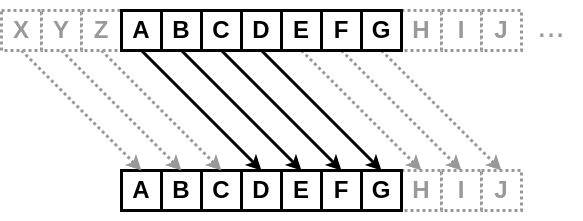
\includegraphics[width=0.4\textwidth]{fig/caesar.png}
	\caption{The method of the Caesar cipher}
	\label{fig-caesar}
\end{figure}

Cryptography has ancient roots, dating back to antiquity. One of the most basic
techniques is the Caesar cipher (see Fig. \ref{fig-caesar}),
named after Julius Caesar. This method works
by shifting each letter in the plaintext by a fixed number of positions in the
alphabet, with the classic Caesar cipher employing a left shift of three.
Despite its simplicity, this method laid the foundation for more advanced
cryptographic systems. In CTF challenges, basic cryptography problems often
begin with similar (e.g. monoalphabetic) ciphers, offering an introduction
to fundamental concepts
while requiring participants to crack these basic codes through logical
analysis and pattern recognition.
It is also worth to mention base64, hexadecimal base16 and uu encodings,
that are often used to transfer arbitrary binary data through ASCII channels.

More advanced cryptography challenges often exploit vulnerabilities within
specific algorithms or their implementations, such as flaws in key generation
or usage. Successfully tackling these challenges requires a deep understanding
of the mathematical principles underlying the cryptographic techniques.
These
advanced tasks emphasize not just the mechanics of encryption but also the
critical importance of secure implementation in real-world applications.

\subsection{Reverse Engineering}

The goal of reverse engineering is to understand how a program or system (such
as a network service) operates. One classic task involves figuring out the
specific input that will produce a given output. Reverse engineering challenges
generally fall into three main categories.

In the first category, participants are provided with the source code, which
may or may not be obfuscated. The challenges can be written in any programming
language (such as Python, C, JavaScript, or others). In this scenario,
participants can modify, compile, and test the code with various inputs,
allowing them to experiment with the program’s behavior.

In the second category, only the binary of the program is provided. Tools like
Ghidra
%Ghidra
\cite{eagle2020}
are particularly useful for these challenges, as they can decompile
binaries into a pseudo C-like code for analysis (see Fig. \ref{fig-ghidra}).
After performing static
analysis, participants can reorganize the generated code, rename automatically
assigned function and variable names, and deduce the program's internal
operations. This process helps them understand how the binary works and
identify potential ways to manipulate or exploit it.


\begin{figure}[htbp]
	\centering
	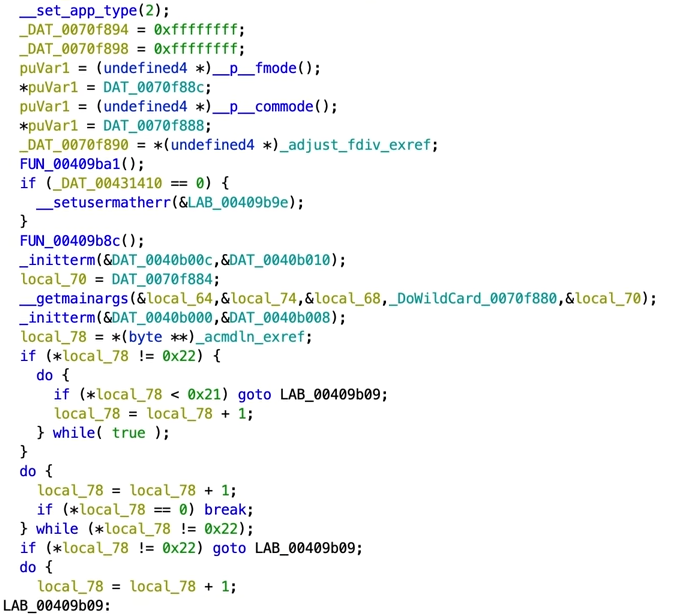
\includegraphics[width=0.4\textwidth]{fig/ghidra.png}
	\caption{Reverse engineering a binary file with Ghidra}
	\label{fig-ghidra}
\end{figure}

The third category involves black-box analysis, where neither the source code
nor the binary is provided. Instead, the program is typically accessible
through a network connection. Participants must deduce the program's internal
workings by systematically providing different inputs and observing the
outputs, uncovering vulnerabilities or hidden functionalities purely through
external interaction.

\subsection{Binary Exploration}

\begin{figure}[htbp]
	\centering
	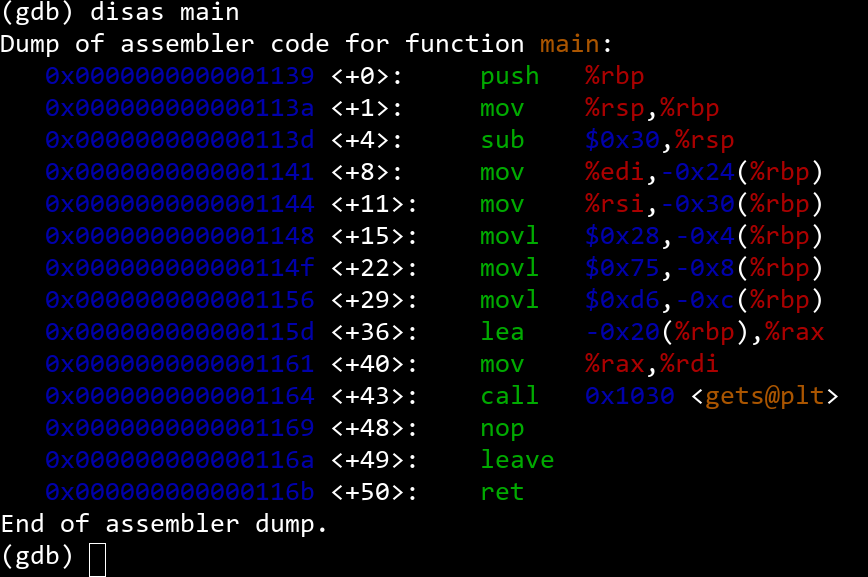
\includegraphics[width=0.4\textwidth]{fig/gdb.png}
	\caption{Disassembling a binary function in GDB}
	\label{fig-gdb}
\end{figure}

Binary exploitation is a classic technique used to create exploits for binary
programs, i.e. to give a specially crafted input, that redirects the flow
of the program to call a given function, or execute an attacker code.
In these challenges, participants analyze executable files to
identify vulnerabilities such as stack or buffer overflows
%Buffer overflow
\cite{lhee2003}
or format string
vulnerabilities.
Modern compilers and operating systems implement various countermeasures,
including stack canaries and address space layout randomization (ASLR), which,
in case of particular challenges,
must also be bypassed to successfully exploit the program. To aid participants, some
challenges also provide the program’s source code, offering additional insight
into the vulnerability.

Solving these types of challenges typically requires running the program
step-by-step, inspecting variables, and examining the state of the stack and
registers during execution. One of the most powerful tools for this process is
the GNU Debugger (GDB)
%GDB
\cite{stallman1988},
which allows participants to perform detailed analysis and manipulation of
the program during runtime. By using GDB, participants can gain a better
understanding of how the binary operates, identify critical points of
exploitation, and craft effective payloads to take control of the program.
Fig. \ref{fig-gdb} shows a screenshot of GDB after partially disassembling
the main function of the investigated binary executable.

\subsection{Forensics}

Similar to real world (digital) forensyscs, when, during an investigation,
the seized IT equipment must be analyzed to find evidence. The usually
asked questions: Was this file (content) present on a storage device?
Was some file deleted? What is the real date of a file? Who is the real sender
of an e-mail? Was this file transferred from this to that computer?

Filesystem, or complete storage media image, which contain the state of the system at a particular
time. Can be booted, but this data is extremely fragile and the live system
can destroy the traces / evidences. Important to investigate the system without
modifying it. Hidden partition, deleted file.

Another possible task is to analyze network traffic. Understand network
protocols. Wireshark.

Sometimes only a few files (e.g. a webpage) must be analyzed. Metadata,
digital signatures.

Another possible forensics problem can be connected to steganography.
Steganography is the art of hiding data without an actual encryption.
This technique allows arbitrary data, such as strings or files, to be hidden
within other media, like image files, without raising suspicion.
Modern software tools implement steganography by manipulating the least
significant bits (LSBs) of pixel values in an image. This method enables data
to be embedded in a way that is imperceptible to the naked eye, as the changes
made to the pixel values are minimal and often unnoticeable.


%Steganography
\cite{morkel2005}



\begin{figure}[htbp]
	\centering
	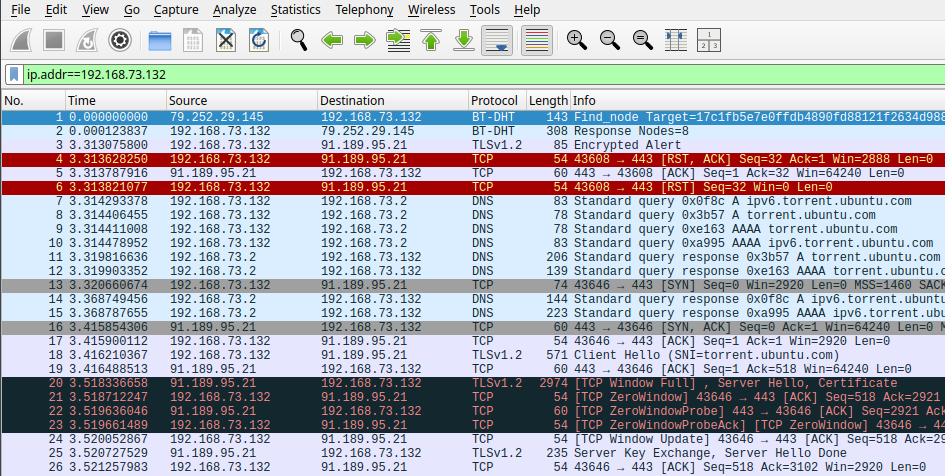
\includegraphics[width=0.5\textwidth]{fig/wireshark.png}
	\caption{Analyzing network traffic with Wireshark}
	\label{fig-wireshark}
\end{figure}


%Wireshark forensics
\cite{ndatinya2015}


\subsection{Miscellaneous}

Misc, which does not fit anywhere else.
The problem can be connected to file formats. To fix the corrupted file (e.g. the file header)
to display it.

Many file formats allow parts in them, which are not executed, or displayed. This opens
the possibility to hide data or another file. Important to detect the signs (e.g. the
magic bytes) of particular files.

Binwalk is a good tool to automatically analyze and extract files, but sometimes it is
not able to identify the contents.

Polyglot can be interpreted as different files, e.g. pdf and png with different
content.

A special subject is IoT and embedded security. There, besides the mentioned
types, another, special vulnerabilities are exists. Power analysis / side channel
attack, fault injection.

%IoT vulnerabilities
\cite{butun2019}

%Fault injection
\cite{ziade2004}


\section{Summary}

Capture the Flag (CTF) challenges offer a highly effective way of developing
essential cybersecurity skills by providing hands-on experience in a
competitive, gamified environment. This article explores how CTFs function as
both educational tools and recruitment platforms, emphasizing their role in
making cybersecurity more accessible to beginners while offering advanced
participants opportunities to deepen their expertise. By analyzing popular CTF
events like DEF CON, picoCTF, and Google CTF, the article highlights how these
competitions engage participants with real-world cybersecurity problems, thus
fostering critical problem-solving abilities. Furthermore, it examines how CTFs
contribute to both individual skill development and the broader cybersecurity
community.

\bibliographystyle{IEEEtran}
\bibliography{IEEEabrv,references}

\end{document}
